\section{Model architecture}
\label{model_architecture}

\begin{figure}
\centerline{
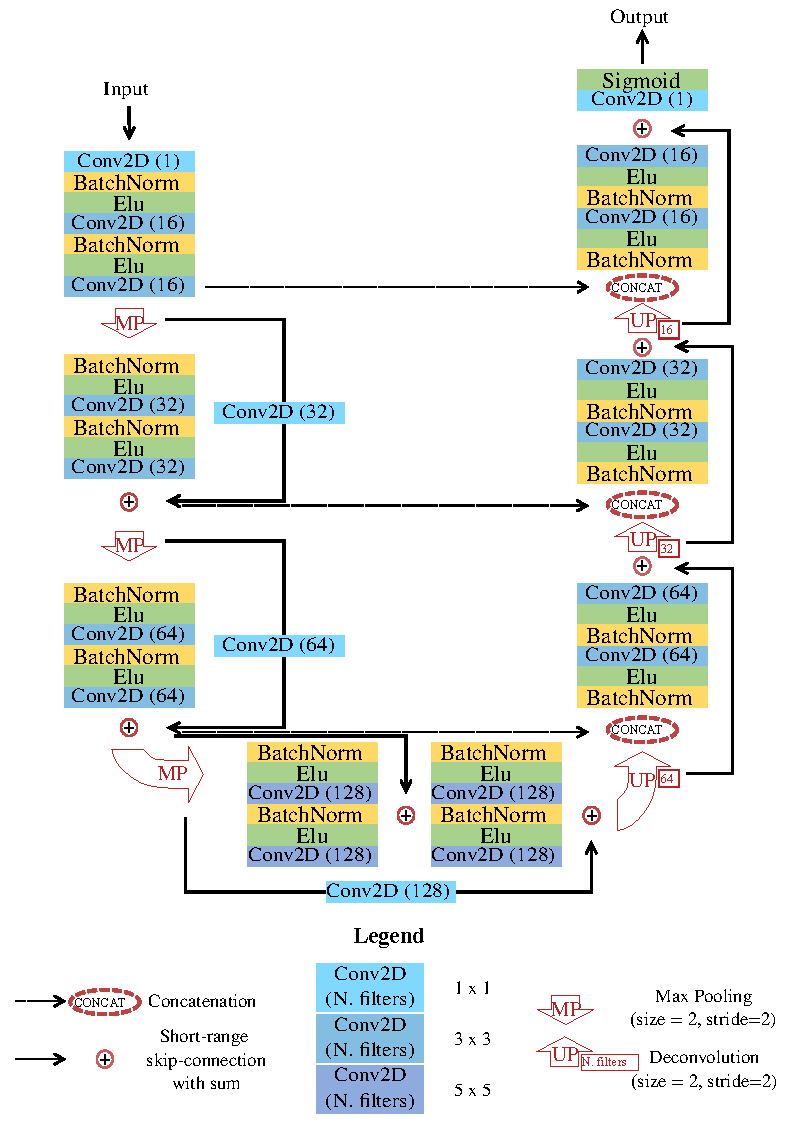
\includegraphics[width=0.8\textwidth]{figures/130_methods/c-resunet_architecture.pdf}
}
\caption{\textbf{Model architecture}. Each box reports an element of the entire architecture (individual descriptions in the legend). 
% The shortcut-connections along the encoding-path are supported by a 1$\times$1 convolution to enable the final sum before the max-pooling operation.
} \label{fig:model_architecture}
\end{figure}
We compare the detection and counting performance of four alternative architectures derived from two network families -- Unet and ResUnet -- commonly used for segmentation tasks.
In the former family, we pick the original Unet architecture \cite{unet} and a smaller version (small Unet) obtained by setting the initial number of filters equal to the ResUnet proposed in \citeA{deep_resunet} and scaling the following blocks consequently.
In the latter, we pick a ResUnet implementation presented in \citeA{deep_resunet} and a similar version with minor modifications.
Specifically, we add an initial 1$\times$1 convolution to simulate an RGB to grayscale conversion.
The advantage of doing so -- as opposed to apply a standard grayscale conversion -- is that the transformation is learned during training so to improve the segmentation performance.
As a further modification, we insert an additional residual block having 5$\times$5 filters -- instead of 3$\times$3 -- at the end of the encoding path. This adjustment should provide the model with a larger field of view, thus fostering a better comprehension of the context surrounding the pixel to classify.
This kind of information can be beneficial, for example, when cells clump together and pixels on their boundaries have to be segmented. 
Likewise, the analysis of some background structures (\cref{fig:dataset:bright,fig:artifacts:stripe,fig:artifacts:macaroon}) can be improved by looking at a broader context.
The resulting architecture is reported in \cref{fig:model_architecture} and it will be referred to as \textbf{cell ResUnet (c-ResUnet)} hereafter.